\documentclass[../../tc_tp5_main.tex]{subfiles}

\begin{document}

%capítulo
\chapter{Celda Universal}

Las celdas universales son filtros que basan su funcionamiento en etapas de integradores, derivadores y sumadores. Esto permite crear circuitos de segundo orden.

\begin{figure}[H]	
	\centering
	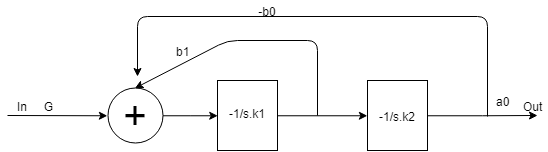
\includegraphics[width=0.6\textwidth]{imagenes/uniGen.png}
	\caption{Celda universal generica}\label{fig:unigen}
\end{figure}

La figura \ref{fig:unigen} muestra una primera aproximación a una celda universal, cuya función transferencia es la siguiente:
$$ H(S)=\frac{S^2 K_1 K_2 }{S^2 K_1 K_2 + b_1 S K_2 + b_0 }$$
De esta ecuación se obtiene $Q$ y $\omega_0$:

$$\omega_0=\sqrt{\frac{b_0}{K_1 K_2}}$$
$$Q=\frac{1}{b_1}\sqrt{\frac{b_0 K_1}{K_2}}$$

Las sensibilidades de $Q$ y $\omega_0$ son:
$$ S^{\omega_0}_{b_0}=\frac{ \partial \omega_0}{\partial b_0} \frac{b_0}{\omega_0}= \frac {1}{2}$$

$$ S^{\omega_0}_{K_1}= S^{\omega_0}_{K_2}= - S^{\omega_0}_{b_0}= -\frac {1}{2}$$

$$ S^{Q}_{b_0}=\frac{ \partial Q}{\partial b_0} \frac{b_0}{Q}= \frac {1}{2}$$

$$ S^{Q}_{K_1}= S^{Q}_{K_2}= S^{Q}_{b_0}= \frac {1}{2}$$

La sensibilidad de $Q$ y $\omega_0$ frente a sus parámetros es constante e igual (en m\'odulo) para todos los par\'ametros que la definen. Esto es una característica favorables de las celdas universales: su baja sensibilidad le permite lograr valores de $Q$ altos.

\section{Comparación de celdas universales}

\subsection{Kerwin Huelsman Newcomb (KHD)}
El circuito correspondiente a esta celda es:

\begin{figure}[H]	
	\centering
	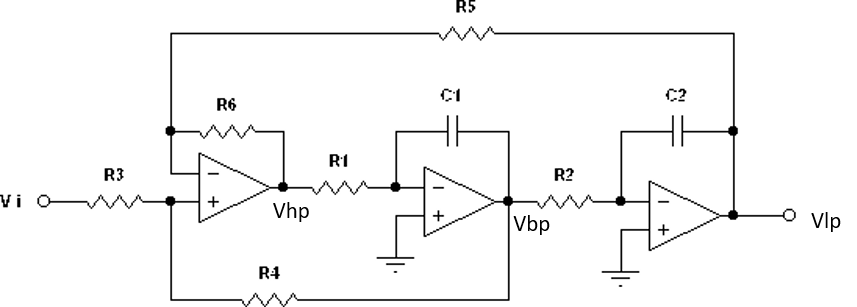
\includegraphics[width=0.6\textwidth]{imagenes/KHN.png}
	\caption{KHN}
\end{figure}

De la cual se obtienen las siguientes ecuaciones:
$$ V_{BP}=- \frac{V_{HP}}{R_1 C_1  S} $$
$$ V_{LP}= - \frac{V_{BP}}{R_2 C_2 S}=\frac{V_{HP}}{S^2 R_1 C_1 R_2 C_2} $$
$$\frac{V_{HP}}{V_i}=  \frac{\frac{R_4}{R_3 + R_4}}{\frac{R_3}{R_3 + R_4} \frac{1}{R_1 C_1 S} + \frac{R_5}{R_5 + R_6} + \frac{R_6}{R_5 +R_6}\frac{1}{S^2 R_1 C_1 R_2 C_2} }$$

De esta \'ultima ecuación se obtienen los valores de $Q$ y $\omega_0$:
$$\omega_0=\sqrt{\frac{\frac{R_6}{R_5}}{R_1 R_2 C_1 C_2}} $$
$$ Q=\frac{\left( 1+\frac{R_4}{R_3} \right) \sqrt{R_6 R_1 C_1}}{\left( 1 + \frac{R_6}{R_5} \right) \sqrt{R_5 R_2 C_2} } $$

En cuanto a la sensibilidades de los par\'ametros anteriormente descriptos en funci\'on de sus componentes, las mismas son:
$$ S_{R_1}^{\omega_0}=S_{R_2}^{\omega_0}=S_{R_5}^{\omega_0}=S_{C_1}^{\omega_0}=S_{C_2}^{\omega_0}=-S_{R_6}^{\omega_0}=\frac{1}{2} $$
$$ S_{R_1}^{Q}=S_{C_1}^{Q}= -S_{R_2}^{Q}=S_{C_2}^{Q}=\frac{1}{2}$$
$$ S_{R_4}^{Q}=-S_{R_3}^{Q}=\frac{R_4}{R_4 +R_3} < 1$$
$$ S_{R_5}^{Q}=-S_{R_6}^{Q}=\frac{-Q}{2}\frac{R_5 - R_6}{1 + \frac{R_4}{R_5}} $$
Si $R_5=R_6$ se logra reducir significativamente la sensibilidad de Q. Dicha baja sensibilidad es una de las mejores caracter\'isitcas de esta celda.



\subsection{Tow Thomas}
El circuito correspondiente a la celda es:
\begin{figure}[H]	
	\centering
	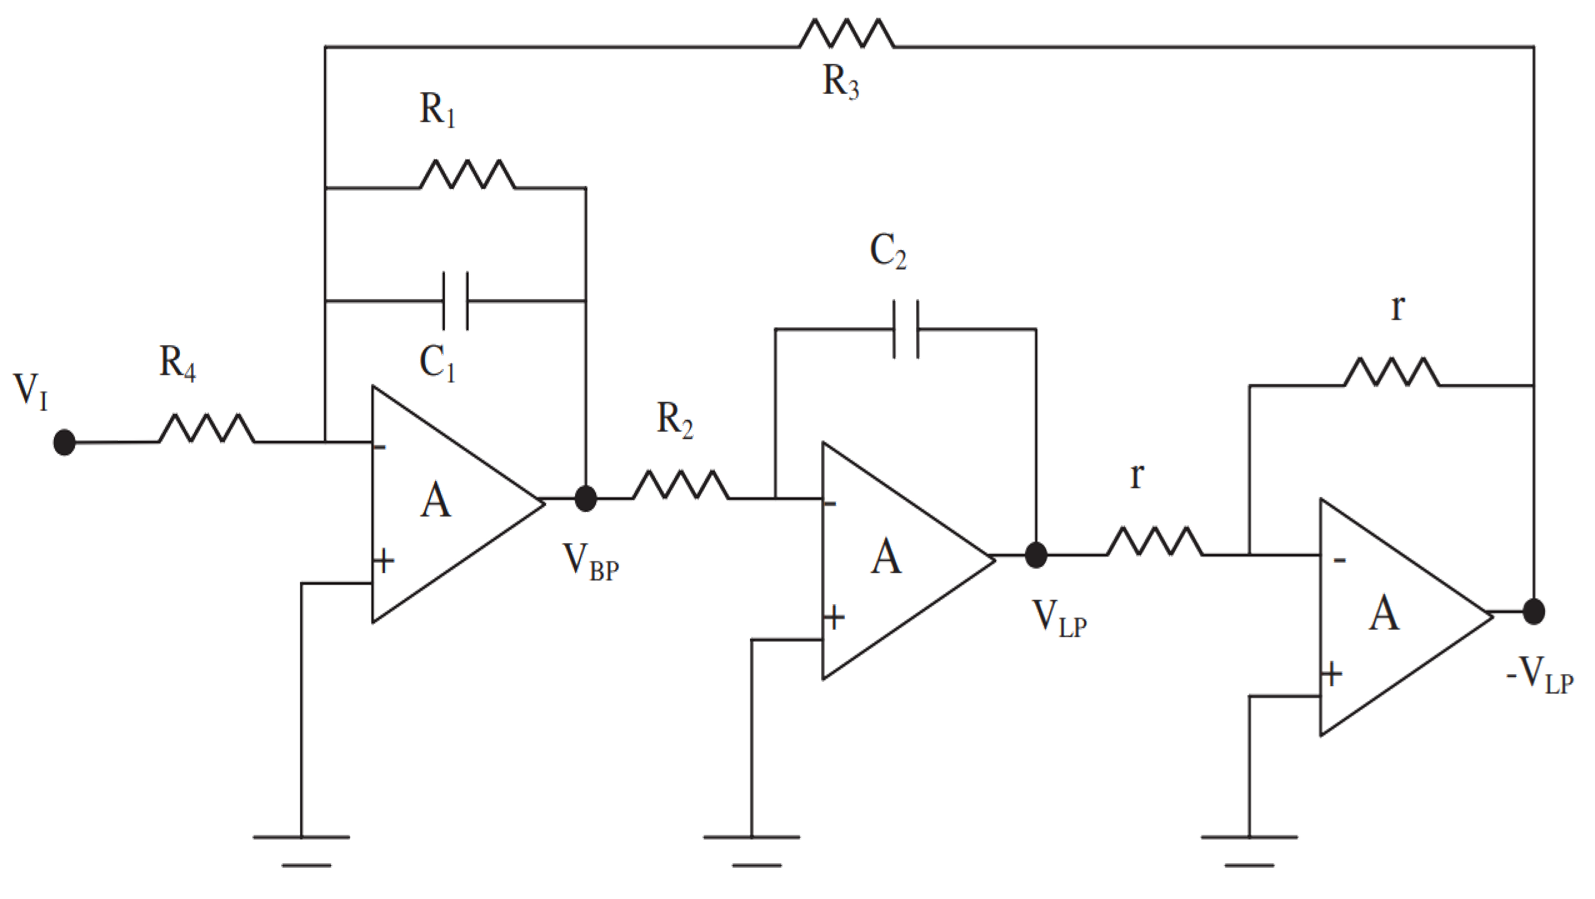
\includegraphics[width=0.6\textwidth]{imagenes/tt.png}
	\caption{Tow Thomas}
\end{figure}

$$\frac{V_{BP}}{V_i}=-\frac{\frac{1}{R_4 C_1}S}{S^2 +\frac{1}{R_1 C_1}S+\frac{1}{R_2 R_3 C_1 C_2}}$$
$$\frac{V_{LP}}{V_i}=\frac{\frac{1}{C_1 C_2 R_2 R_4}}{S^2 + \frac{S}{C_1 R_1}+ \frac{1}{C_1 C_2 R_2 R_3}} $$

Donde $\omega_0$ y $Q$ son:
$$ \omega_0=\frac{1}{\sqrt{C_1 C_2 R_2 R_3}} $$
$$ Q= R_1 \sqrt{\frac{C_1}{C_2 R_2 R_3}}$$
 
La ventaja de la celda es que permite controlar el $Q$ del circuito variando únicamente la resistencia $R_1$, sin alterar el $\omega_0$ ni la ganancia. También variando $R_4$ se logra variar la ganancia del circuito sin alterar el $Q$ y el $\omega_0$.

\subsection{Akerberg Mossberg}

\begin{figure}[H]	
	\centering
	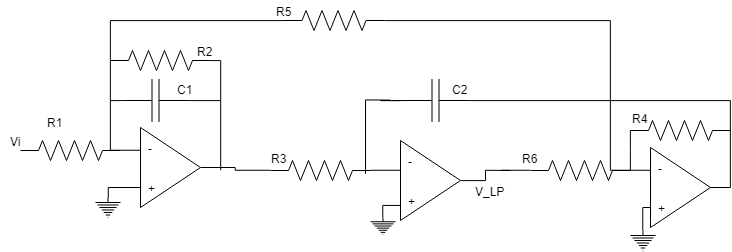
\includegraphics[width=0.6\textwidth]{imagenes/am.png}
	\caption{Akerberg Mossberg}
\end{figure}

Cuya función transferencia es:
$$\frac{V_{Lp}}{V_i}=\frac{\frac{R_5}{R_1}\sqrt{\frac{R_6}{R_3 R_4 R_5 C_1 C_2}}}{S^2 + \frac{1}{R_2 C_1}} $$

De esta expresión se obtiene:

$$\omega_0=\sqrt{\frac{R_6}{R_3 R_4 R_5 C_1 C_2}} $$
$$Q=R_2 C_1 \sqrt{\frac{R_6}{R_3 R_4 R_5 C_1 C_2}}  $$


\subsection{Fleischer Tow}

\begin{figure}[H]	
	\centering
	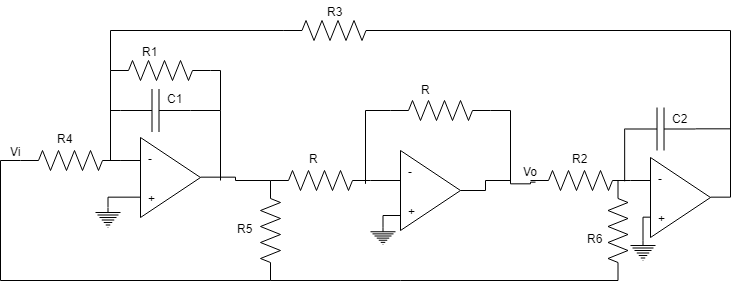
\includegraphics[width=0.6\textwidth]{imagenes/ft.png}
	\caption{Fleischer Tow}
\end{figure}
 
Su función transferencia es la siguiente:

$$\frac{V_O}{V_i}=-\frac{\frac{R}{R_5}S^2 + \frac{1}{R_1 C_1} \left( \frac{R}{R_5} - \frac{R_1}{R_4} \right) S + \frac{1}{R_3 R_6 C_1 C_2}}{S^2 + \frac{1}{R_1 C_1} S +\frac{1}{R_2 R_3 C_1 C_2}} $$

Donde $\omega_0$ y $Q$ son:
$$\omega_0=\sqrt{\frac{1}{R_2 R_3 C_1 C_2}} $$
$$Q=R_1 \sqrt{\frac{C_1}{R_2 R_3 C_2}}$$

Para lograr distintos filtros se utilizan las siguientes condiciones:
\subsubsection{Pasa bajos}
$R_4=\infty$ , $R_5=\infty$ y $R_6=\frac{R_2}{G}$
\subsubsection{Pasa banda}
$R_5=\infty$ , $R_6=\infty$ y $R_4=\frac{R_1}{G}$
\subsubsection{Pasa altos}
$R_6=\infty$ , $R_4=\frac{R_1}{G}$ y $R_5=\frac{R}{G}$
\subsubsection{Rechaza banda}
$ R_4=\frac{R_5 R_1}{R}$
\subsubsection{Pasa todo}
 $R_5=\frac{R}{G}$ ,  $R_6=\frac{R_2}{G}$ y $R_6=\frac{R_1}{G}$


\section{Elaboración del filtro}

\subsection{Plantilla a realizar}
El objetivo del filtro es que cumpla las siguientes condiciones:
\begin{table}[H]
\begin{center}
\begin{tabular}{|l|l|}
\hline
$f_{\infty}$& $30KHz$\\
\hline \hline
$\Delta f_a$ &600Hz  \\ \hline
$\Delta f_p$ &13.2KHz  \\ \hline
$A_a$ &40dB\\ \hline
$A_p$ &6dB\\ \hline
$\abs{Z_{in}(f)}$ & >50$K\Omega $\\ \hline
Filtro & BR\\ \hline



\end{tabular}
\caption{Plantilla} 
\end{center}
\end{table}




\subsection{Elección de celda}
Como el filtro solicitado es un rechaza banda, se necesita que la celda posea una salida pasa altos o rechaza banda. Por ende, como  la celda Tow Thomas y la Akerberg Mossber no las poseen fueron descartadas como opciones. En cuanto a la KHN, para realizar la salida rechaza banda se necesita un sumador, y por lo tanto se eligió la Flesher Tow, que posee una configuración pasa banda sin alterar el circuito (una sola etapa).

\subsection{Analisis de sensibilidades de la celda Fleischer Tow}
Se realizó el c\'alculo de las sensibilidades relativas de $Q$ y $\omega_0$ respecto a sus componentes.
$$S^{\omega_0}_{R_2}=S^{\omega_0}_{R_3}=S^{\omega_0}_{C_1}=S^{\omega_0}_{C_2}=- \frac{1}{2}$$
$$S^{Q}_{R_1}= 1$$
$$S^{Q}_{R_2}=S^{Q}_{R_3}=S^{Q}_{C_2}=-S^{Q}_{C_1}=-\frac{1}{2} $$
Como se observa en las sensibilidades, son constantes y no dependen de los componentes. Esto permite que la celda alcance altos $Q$.


\subsection{Diseño del filtro}
A partir de la plantilla indicada anteriormente, se obtuvieron los valores de las frecuencias de atenuación y de paso $ f_A^-=29701Hz $, $f_A^+=30301Hz $, $ f_P^-=24100Hz $ y $ f_P^+=37344Hz $. Tambien se simuló la función transferencia:
\begin{figure}[H]	
	\centering
	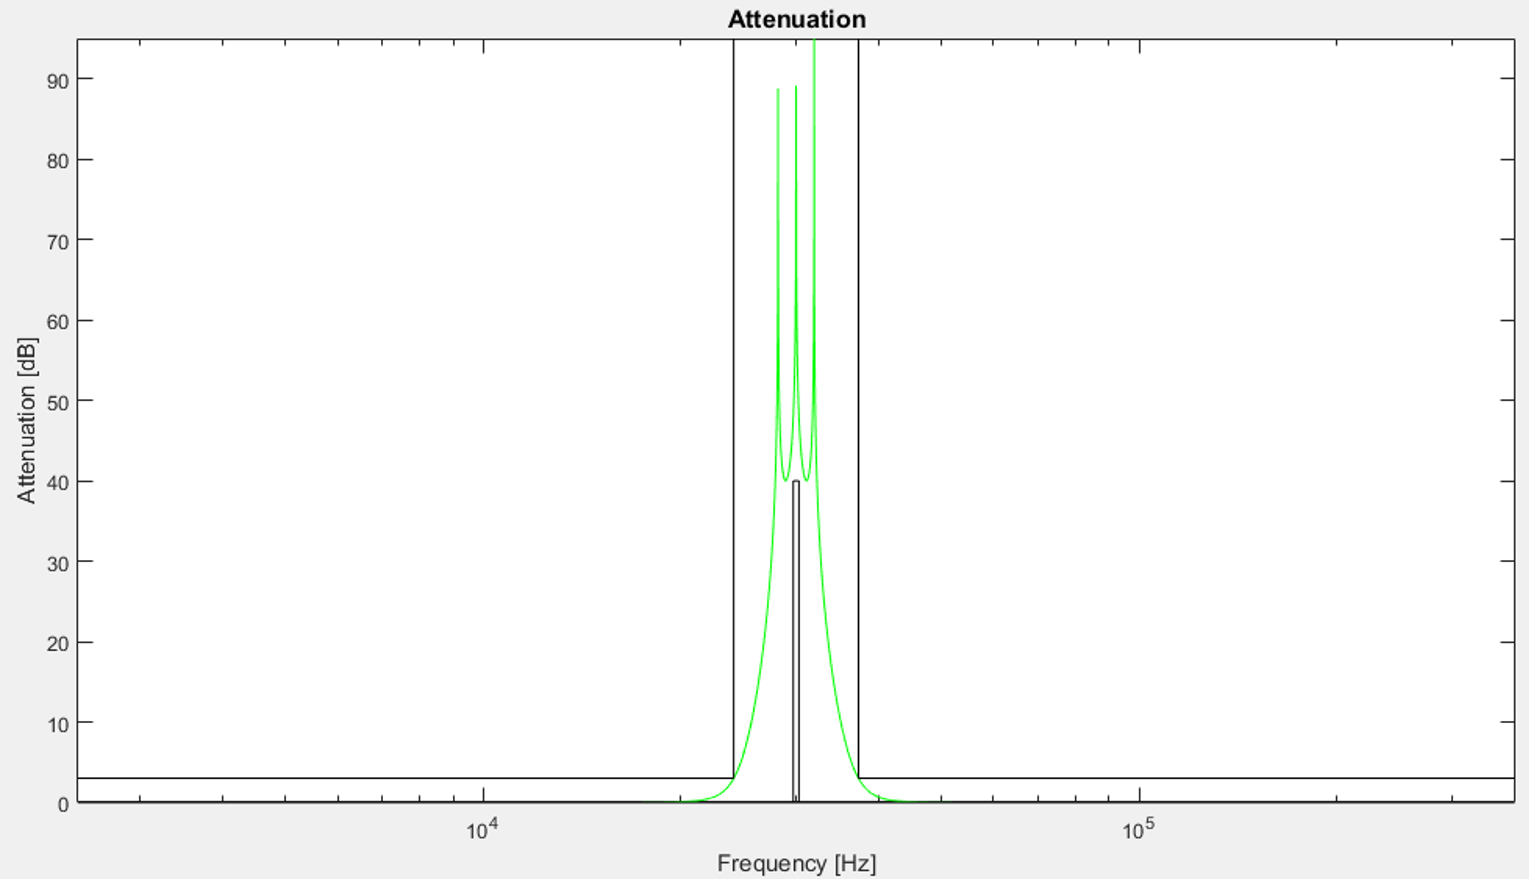
\includegraphics[width=0.4\textwidth]{imagenes/atten.png}
	\caption{Grafico de atenuación}
\end{figure}
\begin{figure}[H]	
	\centering
	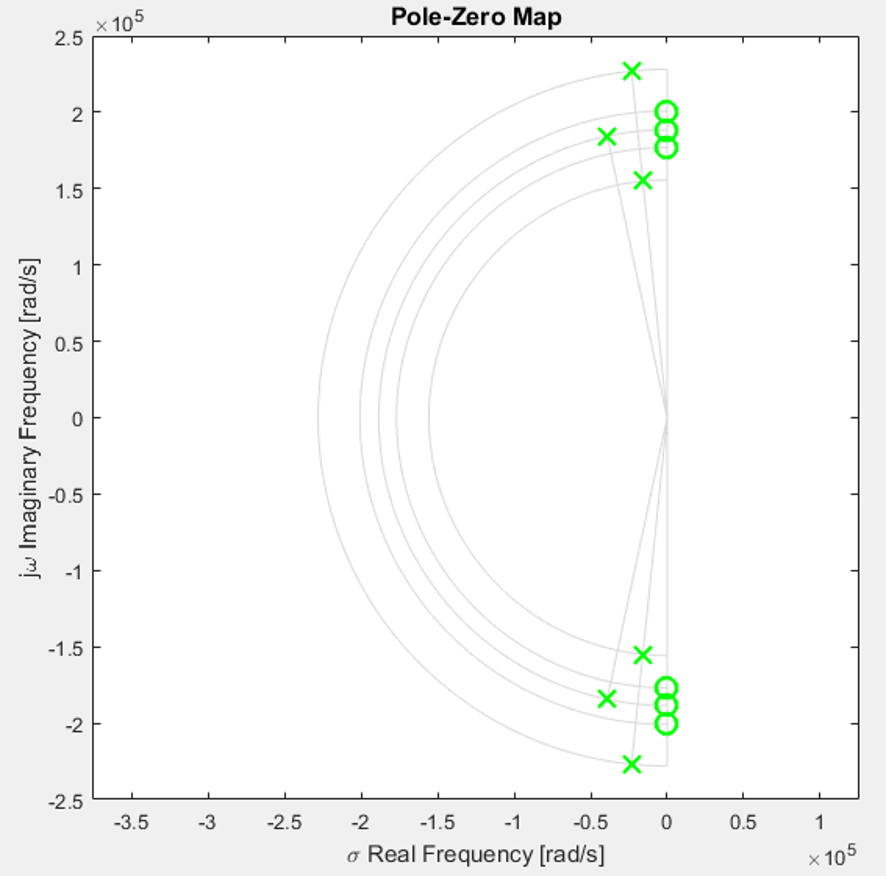
\includegraphics[width=0.4\textwidth]{imagenes/polezero.png}
	\caption{Grafico de polos y ceros}
\end{figure}
A partir de los polos y ceros obtenidos, se eligieron los componentes de las tres etapas necesarias para realizar el filtro.

\subsection{Simulación del modulo del la respuesta en frecuencia}
Se simularon las tres etapas en cascada para corroborar que cumpla plantilla el diseño te\'orico. La tolerancia de las resistencias fueron del 5\% y 10\% para los capacitores.
\begin{figure}[H]	
	\centering
	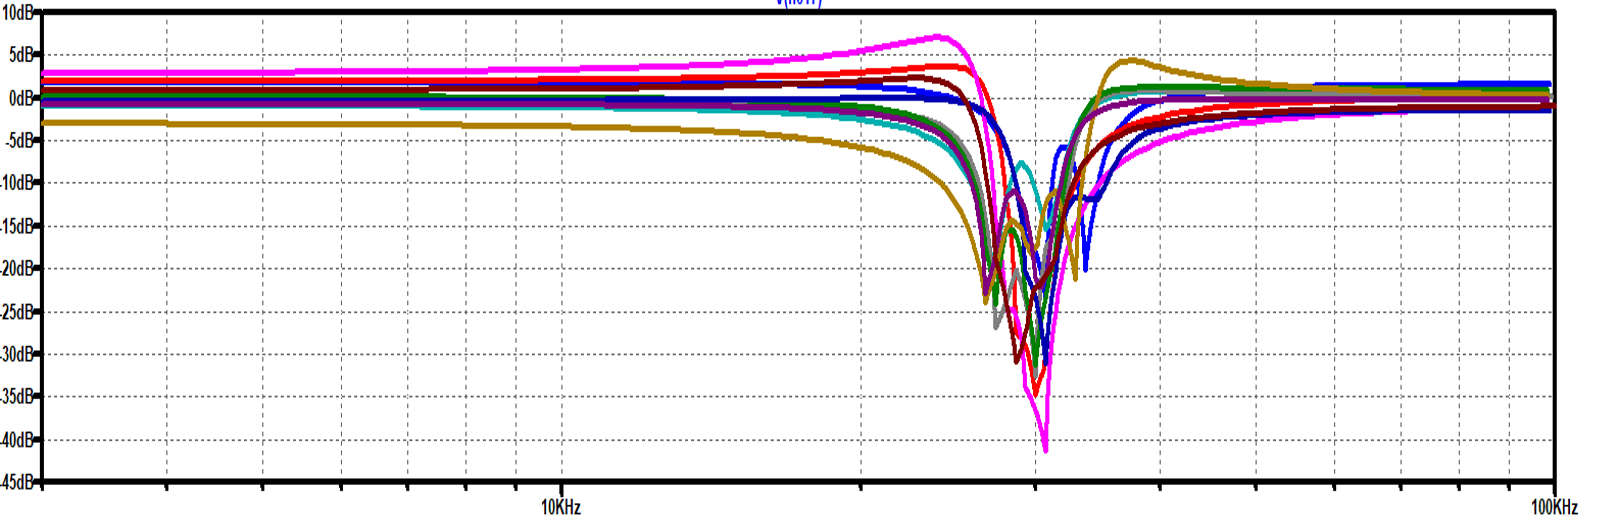
\includegraphics[width=0.8\textwidth]{imagenes/montecarlo.png}
	\caption{M\'odulo de la respuesta en frecuencia}
\end{figure}
Como se observa en la simulación, $f_0\in (28KHz,32KHz)$. Adem\'as se presentan sobrepicos en ganancia: estos se deben a que se deja de cumplir la condici\'on para que las celdas sean pasa banda $R_4=\frac{R_5 R_1}{R}$ y los polos se alejan de los ceros.

A partir del análisis de Montecarlo del circuito se realizó un histograma para conocer la dispersión de las características relevantes del circuito.

\begin{figure}[H]	
	\centering
	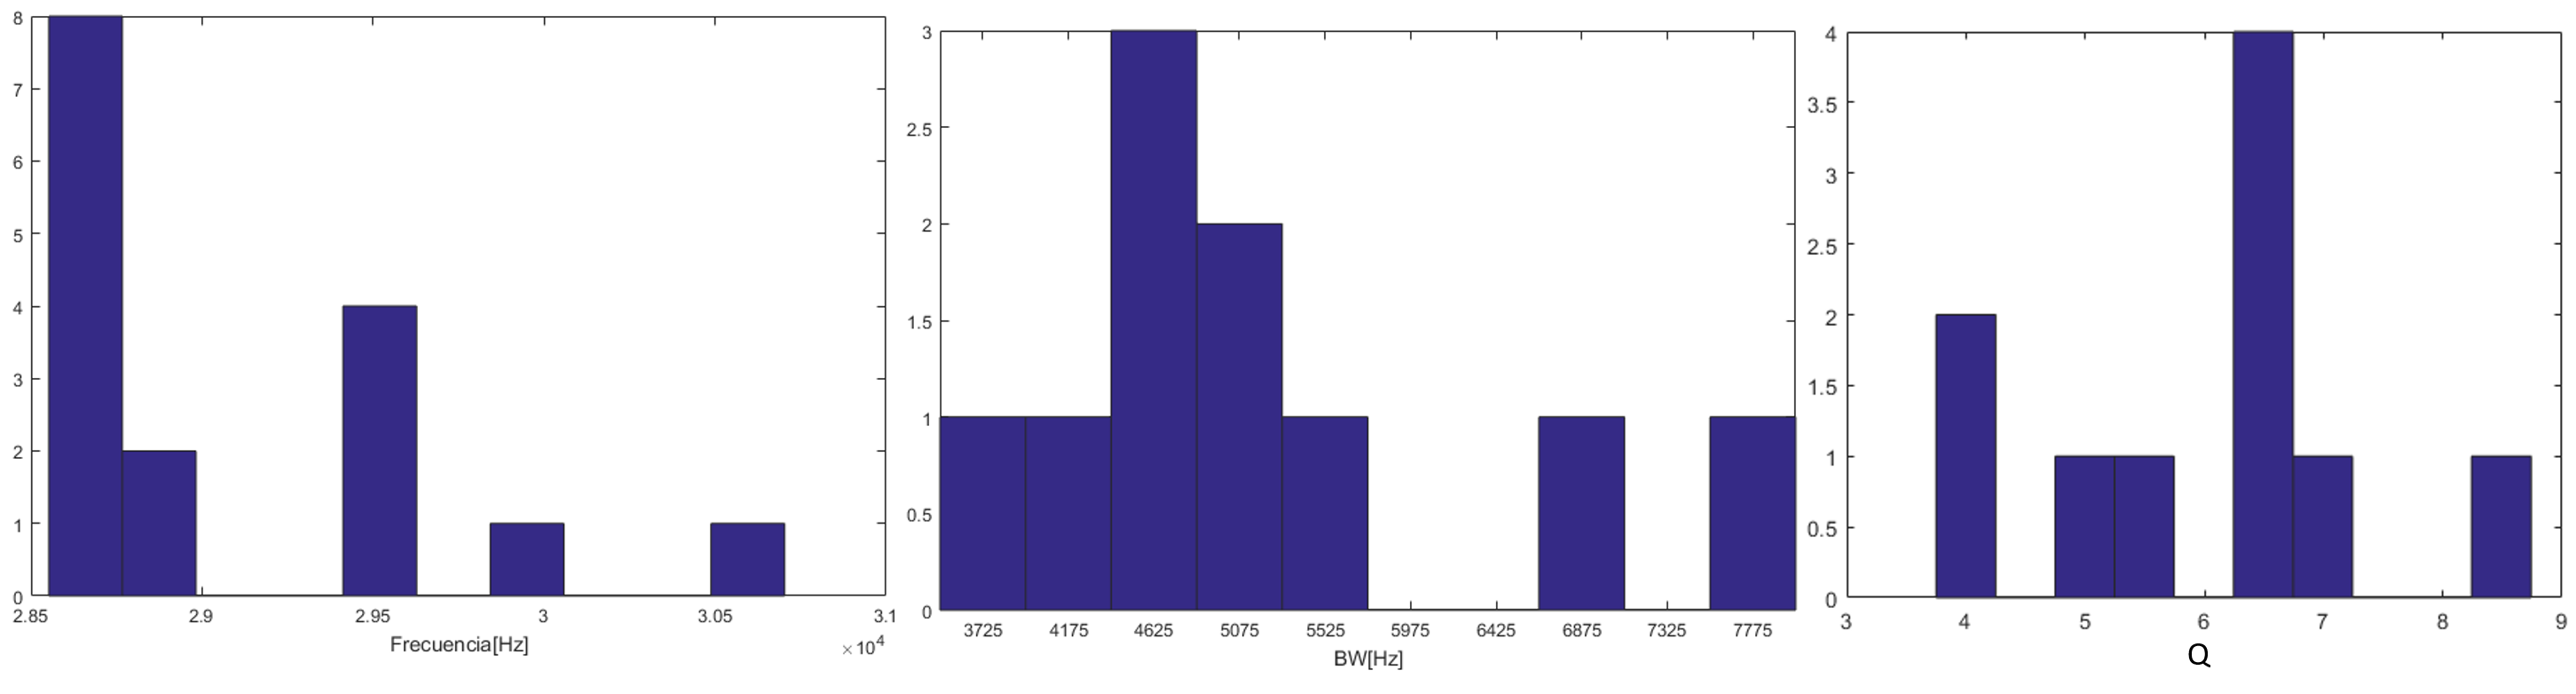
\includegraphics[width=0.95\textwidth]{imagenes/hist.png}
	\caption{Histogramas de $\omega_0$,$\Delta \omega$ y $Q$, obtenidos del analisis de montecarlo}
\end{figure}

\begin{table}[H]
\begin{center}
\begin{tabular}{|l|l|l|}
\hline
 &Valor medio &Desv\'io estándar\\
\hline \hline

$ f_0$ &29161 Hz &621 Hz  \\ \hline
$\Delta f$ & 5166 Hz&1378 Hz  \\ \hline
$Q$ &5.6 &1.42  \\ \hline

\end{tabular}
\caption{Información estadística del análisis de Montecarlo} 
\end{center}
\end{table}

\subsection{Simulación de la impedancia de entrada}
Como se observa en la figura, la impedancia de entrada del circuito es menor que $7K\Omega$. Por ende, para conseguir una impedancia de entrada superior a los $50K\Omega$, al filtro se le agreg\'o un buffer.

\begin{figure}[H]	
	\centering
	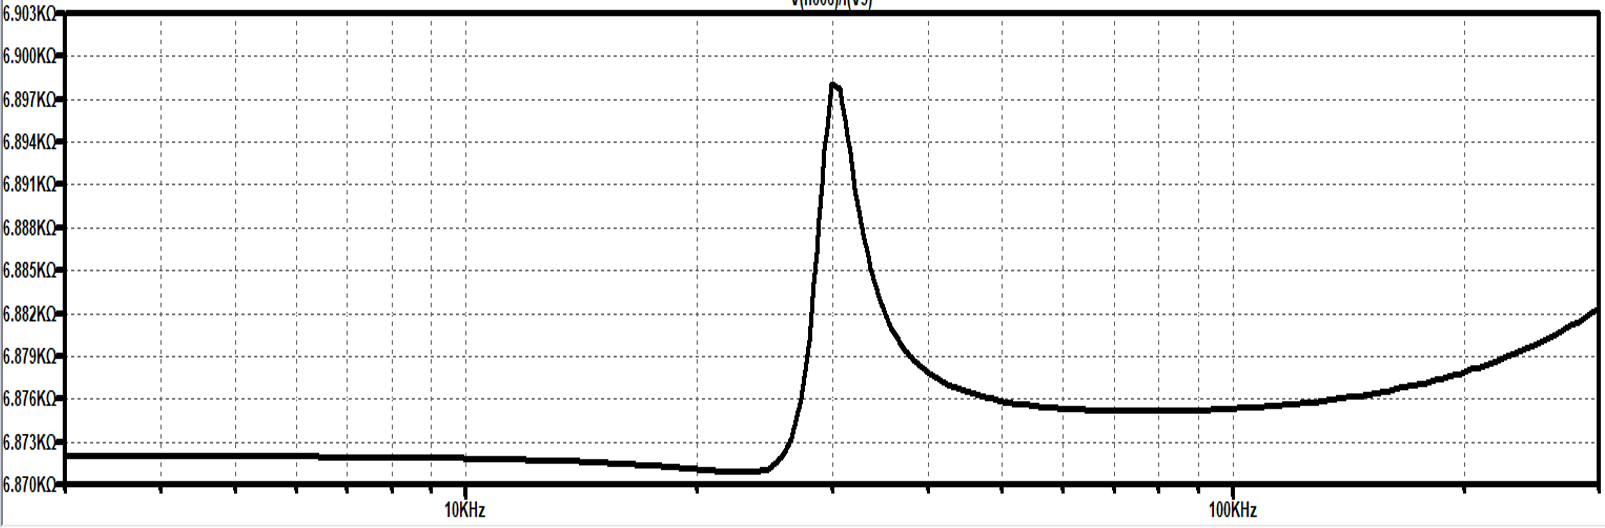
\includegraphics[width=0.9\textwidth]{imagenes/zinsim.png}
	\caption{Simulación de la impedancia de entrada}
\end{figure}


\subsection{Mediciones}

Se midió la respuesta en frecuencia y la impedancia de entrada del circuito.

\begin{figure}[H]	
	\centering
	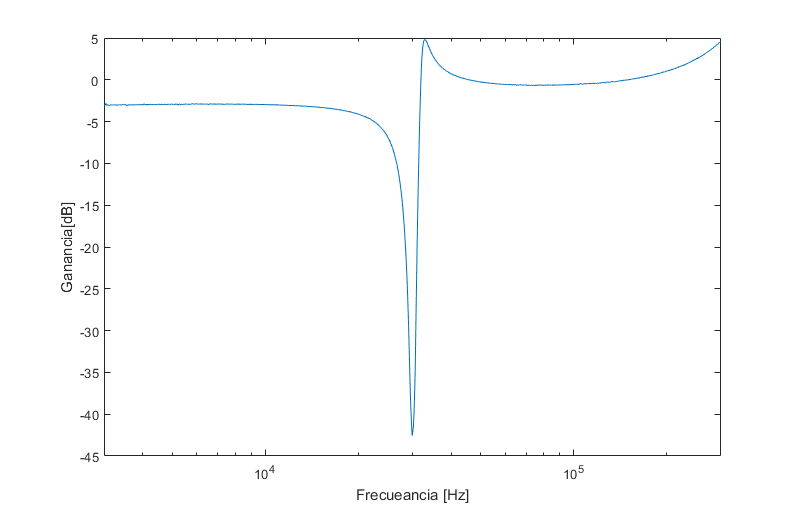
\includegraphics[width=0.6\textwidth]{imagenes/mag.png}
	\caption{M\'odulo de la respuesta en frecuencia}
\end{figure}

\begin{figure}[H]	
	\centering
	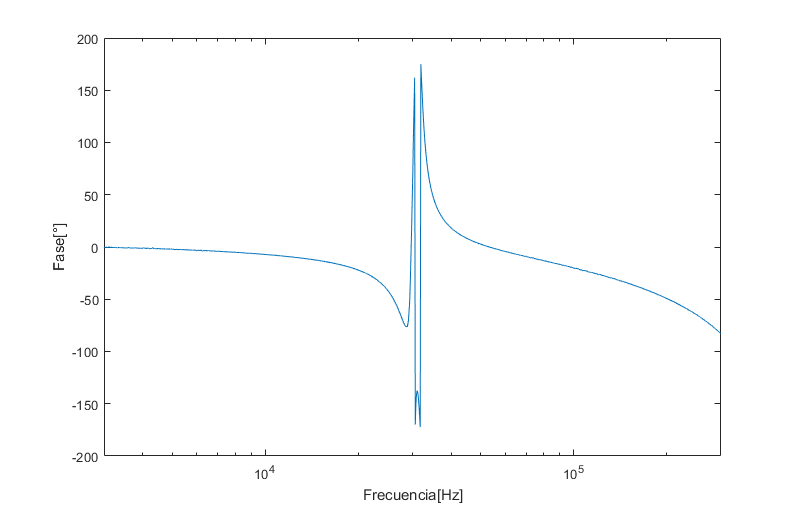
\includegraphics[width=0.6\textwidth]{imagenes/fase.png}
	\caption{Fase de la respuesta en frecuencia}
\end{figure}

\begin{figure}[H]	
	\centering
	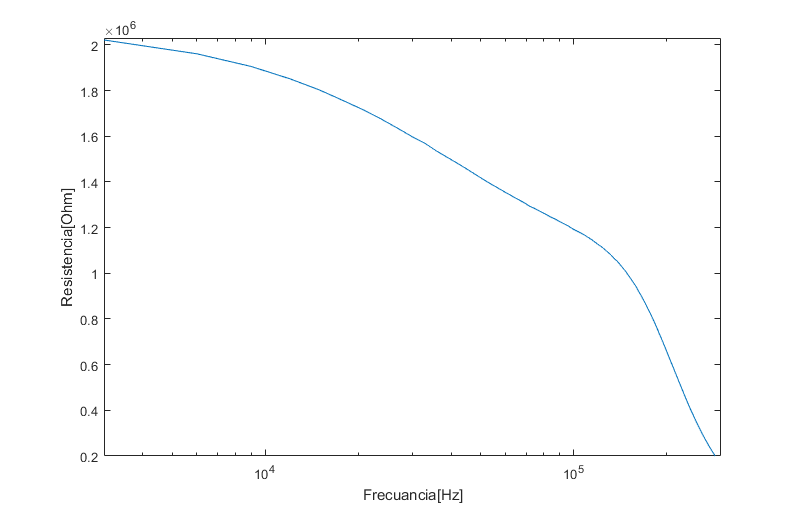
\includegraphics[width=0.6\textwidth]{imagenes/zinMag.png} 
	\caption{M\'odulo de la impedancia de entrada}\label{fig:zinmagg}
\end{figure}


\begin{figure}[H]	
	\centering
	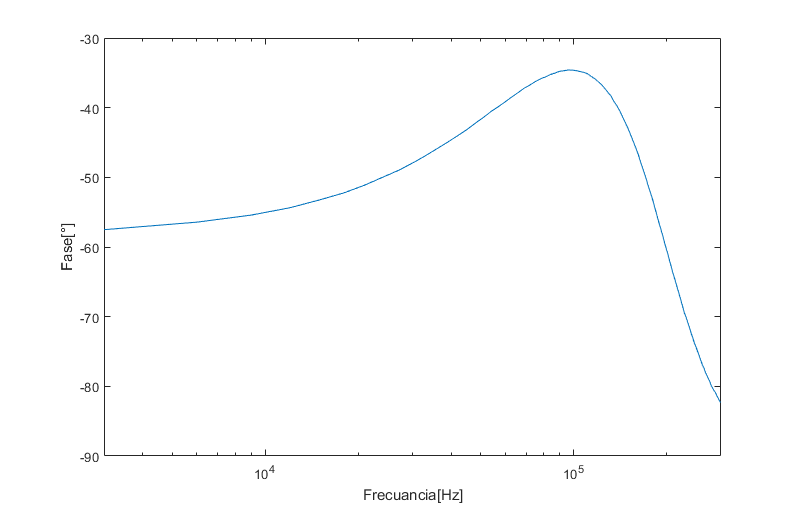
\includegraphics[width=0.6\textwidth]{imagenes/zinFase.png}
	\caption{Fase de la impedancia de entrada}
\end{figure}
Tal como se observa en gr\'afico \ref{fig:zinmagg}, la impedancia de entrada supera los $50K\Omega$, por ende se cumple la condición de diseño solicitada.

Al grafico de la respuesta en frecuencia se le superpuso la plantilla indicada anteriormente. Para observar correctamente la plantilla y la respuesta en frecuencia, se midió en un intervalo de frecuencias cercanas al sobre pico.

\begin{figure}[H]	
	\centering
	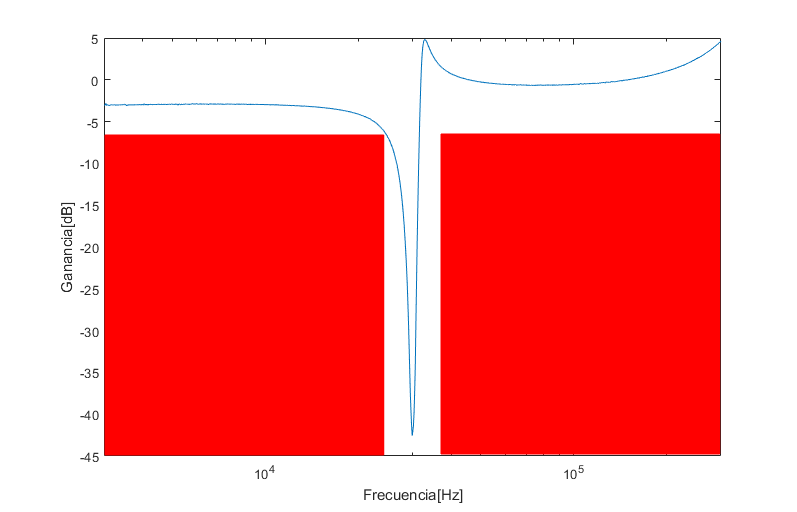
\includegraphics[width=0.6\textwidth]{imagenes/magplant.png}
	\caption{M\'odulo de la respuesta en frecuencia y plantilla}
\end{figure}

\begin{figure}[H]	
	\centering
	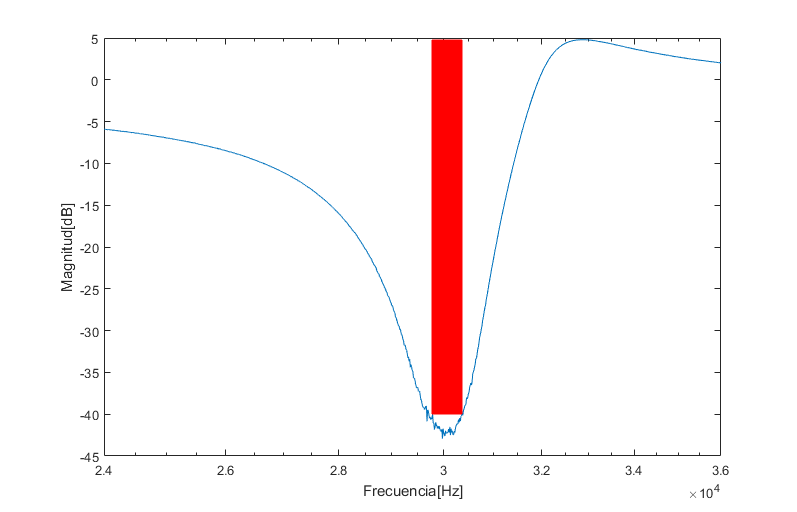
\includegraphics[width=0.6\textwidth]{imagenes/Zmagplant.png}
	\caption{Zoom del m\'odulo de la respuesta en frecuencia y plantilla}
\end{figure}

Tal como se observa en los gráficos previos, se cumple satisfactoriamente la plantilla.



\clearpage\newpage


\end{document}
